\section{Structure from Motion}
\b{Given:} Stereo case extended to more than two cameras by either adding more cameras or moving the same camera in space.\\

\b{Goal:} Estimate camera position AND 3D reconstruction of the scene.\\

\b{Important:} We observe a \b{static} scene from multiple viewpoints \b{over time}.\\

The F-matrix counterpart in the three-point case is called the \b{trifocal tensor} (also available in four-camera case \f{\to} quadrifocal) and describes the constraints for corresponding points in three (or four) cameras. This tensor representation stops for more than four views and we need to handle it differently.\\


\subsection{Overview}
\begin{itemize}
    \item Given the internal camera parameters, the essential matrix \f{E} can be estimated from 2D point correspondences of the camera motion.
    \item Internal camera parameters and essential matrix are sufficient for metric reconstruction.
\end{itemize}
For structure from motion we need:
\begin{itemize}
    \item Internal camera parameters
    \item Sparse point correspondences to estimate \f{E}
    \item Sparse or dense point correspondences to reconstruct scene
    \item An optimization process to couple these processes to refine the result (\f{\to} Bundle Adjustment)
\end{itemize}

\subsection{Bundle Adjustment}
In the general case, we want to optimize the projection matrices \f{P^i} of all cameras and all 3D points \f{X_j} given the image points \f{x_j^i} by minimizing the reprojection error:
\cf{
    \min_{P^i, X_j}\sum_{ij}d^2(P^iX_j, x_j^i)
}
\begin{figure}[h!]
    \centering
    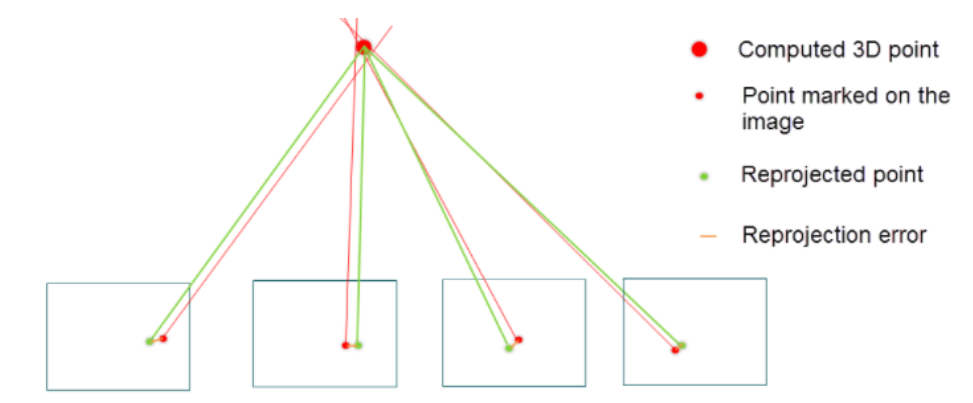
\includegraphics[width=0.5\textwidth]{bundle.png}
\end{figure}

Note that this general case is very sensitive to noise. Knowing the internal camera parameters of each camera, only their rotation \f{R^i} and translation \f{t^i} relative to a reference need to be estimated, which leaves us with:
\cf{
    \min_{R^i, t^i, X_j}\sum_{ij}d^2(P^i(R^i, t^i)X_j, x_j^i)
}
The intuition here is that we need to shift and rotate the bundle of projection rays such that the point distances \f{d(x,y)} get minimized.\\

\b{Advantage:} Bundle adjustment is very flexible with regard to the model. We can even estimate some internal camera parameters by adding them to the term and adding a prior.\\
\b{Drawback:} The cost function is nonlinear and non-convex with many local minima. So we need to get good initialization and then refine using bundle adjustment.\\

\b{Linear BA with Factorization Algorithm\\[.5em]}
The linear bundle adjustment method is based on the affine camera model with 
\cf{
    P=\begin{pmatrix}
        m_{11}&m_{12}&m_{13}&t_1\\
        m_{21}&m_{22}&m_{23}&t_2\\
        0&0&0&1\\
    \end{pmatrix} \quad\to\quad
    \begin{pmatrix}
        x\\y
    \end{pmatrix} = M
    \begin{pmatrix}
        X\\Y\\Z
    \end{pmatrix} + t
}
by which the projection becomes linear. This approach, however, assumes that the depth variation in the scene is small compared to the distance to the camera. In the linear case the reprojection error becomes a simpler problem:
\cf{
    E(M^i, t^i, X_j) = \sum_{ij}||x_j^i-(M^iX_j + t^i)||^2\quad,
}
which leads to \f{t_i = \mu_i = \frac{1}{n}\sum_jx_j^i}. Subtracting the centroid \f{\mu^i} from the sum leads to \f{t^i = 0}, by which the remaining optimization problem becomes a factorization problem:
\cf{
    E(M^i, X_j) = \sum_{ij}||x_j^i-M^iX_j||^2
}
The problem with this factorization method is that it requires creating the measurement matrix \f{W} from all points \f{x_j^i}, so all points must be visible in all cameras, which is bad for large scenes! Using SVD this measurement matrix is the factorized.\\
The solution then however still contains the scale ambiguity of metric reconstruction and the affine ambiguity (\f{W=MAA^{-1}X} for any rank 3 matrix \f{A}). The remove the affine ambiguity we can use metric reconstruction with the internal parameters to compute the position of the camera.\\

\b{Initialization of BA\\[.5em]}
Factorization could provide an initialization for subsets of images where all points are visible in all frames, which is typically unrealistic.\\
More common is to use the minimum subset of two images (where all points are visible) and then add more views incrementally.\\

With only two frames the process is similar to previous chapters: Estimate the essential matrix from point correspondences and factorize it into relative translation and rotation.\\
Then, using transitivity, if we know the motion from frame A to frame B and from B to C, we can get the motion from A to C:
\cf{
    R_{AC} = R_{BC}R_{AB}\qquad,\qquad t_{AC} = R_{BC}t_{AB}+t_{BC}
}

\b{Initial reconstruction:}
\begin{enumerate}
    \item Build projection matrices \f{P^i = K^i(R^it^i)}
    \item Triangulate 3D points \f{X_j} from projection matrices and 2D points
    \item Use constraints from all cameras where point \f{X_j} is visible to solve \f{AX_j=0}
\end{enumerate}
\newpage
\b{Incremental BA\\[.5em]}
If we initialize bundle adjustment well enough and there are points jointly visible in distant images, bundle adjustment is a global optimization that optimally corrects drift (accumulation of errors).\\

To mitigate drift, we can run bundle adjustment after adding a new frame to the chain. Note that this is rather slow and can not run in realtime. \b{Loop-closing} also reduces drift by adding long-distance correspondences but also adds risk of adding more drift in some cases.\\

\b{Optimization\\[.5em]}
With a good initialization, the solution can be refined by minimizing the highly nonlinear reprojection error (from before). The nonlinearity is due to the distance \f{d(x,y)} in image coordinates, which requires division by the third component.\\
Due to outliers, it further makes sense to use a robust norm \f{\Psi(d)}, which would add another nonlinearity.\\
This problem can then be minimized via the \b{Levenberg-Marquardt} method (or Gauss-Newton, but that's not always stable in BA). \\

The Levenberg-Marquardt method is a mixture of Gauss-Newton and gradient descent and guarantees to decrease the energy in each iteration. For the method we need the Jacobian of the cost function:
\cf{
    J^\top = \nabla E(x_j^i)=\frac{\delta E(x_j^i)}{\delta p}
}
Each entry is the derivative of each measured point with regard to the parameters. The Jacobian is quite sparse because each 2D point triggers a dependency only between few parameters.\\

\b{Advantage:} It can deal well with occlusions, as they are simply 0 in the matrix and don't cause additional problems.\\

With \f{\tau^*} being the maximum \f{\tau} for which the energy decreases, the problem can be formalized as:
\cf{
    (J^\top J + \frac{1}{\tau^*}I)\text{dp} + J^\top E=0
}
This adds a regularization constant to the diagonal of the system matrix.\\

\b{Similarity to optical flow:}
\begin{itemize}
    \item Each equation corresponds to a derivative with regard to a camera parameter or 3D coordinate and a specific 2D point \f{x_j^i}
    \item In optical flow it corresponded to the derivative with regard to the u or v component of the flow at a certain pixel and the gray value there
\end{itemize}
\vspace{0.5em}
\b{Benefits of Bundle Adjustment:}
\begin{itemize}
    \item All parameters get globally coupled \f{\to} minimum accumulation of errors
    \item Not an algebraic but the geometric distance is optimized \f{\to} each point is treated equally
    \item Missing points (due to occlusion) are unproblematic
    \item Parameters that were assumed to be known for estimating an initialization can be refined (e.g. focal length, lens effects) \f{\to} Autocalibration
    \item Priors can be added to the cost function
\end{itemize}
\newpage
\b{Applications:} Reconstruct from video, reconstruct from tourist photo collection

\subsection{Depth Map to Surface}
Bundle adjustment already provides camera parameters and a sparse 3D point cloud. Corresponding dense depth maps yield a dense point cloud, not a surface!\\

Depth map fusion globally optimizes the point cloud (in terms of smoothness and outliers) to yield smooth surfaces.\\

DTAM performs camera tracking based on dense depth maps.\\

\b{Left out: DTAM}\\

\b{Camera Tracking\\[.5em]}
Camera tracking is the task of optimizing the pose parameters \f{T_{rj}} (6 d.o.f) to fit the recorded image \f{I_j} to the image \f{\tilde{I}_j} rendered from the depth map:
\cf{
    E(T_{rj}) = \int \left(I_j(x) - \tilde{I}_j(T_{rj}x)\right)^2dx
}
This can be optimized via Gauss-Newton. The advantage is that it only requires optimization for 6 parameters and thousands of pixels. Also, there is no error accumulation due to matching relative to the common depth map of the reference frame.\\

\b{Fast depth estimation} is another process that, for each pixel independently, finds the depth that yields the best matching cost over \f{n} frames.

\subsection{Deep Learning and Structure from Motion}
The problem with normal Encoder-Decoder structures is that the model usually only learns from one image and ignores the other (depth from single image).\\

\b{DeMoN\\[0.5em]}
Consists of a bootstrap net (to combine images) followed by an iterative net, which first estimates optical flow and from that estimates depth and egomotion (iteratively refined), from which a refinement net finally produces the depth map. This network works quite well in non-static scenes.\\

Outputs: Depth image and egomotion\\

\b{DeepTAM\\[0.5em]}
DeepTAM is keyframe based (no drift within keyframe), can be fully learned and self-initialized.\\
From the keyframe you get an image and a depth map from which the virtual keyframes of the new pose of the current frame can be rendered. The network then produces pose increments. It can also utilize optical flow as an auxiliary task during training.

\newpage